  Before we understand how the requests work together, it makes sense to understand their individual behavior, i.e., to consider the case where we make only a certain request, since certain decisions in later testing may be influenced by the behavior we observe in these first tests. For the POST requests, since we encompassed them all in one task, we consider all 4 as one type, and due to the heavy computation (4 different requests, as well as the random generation of the dataset and file to be uploaded to the platform), we chose to run only up to 100 users, which will serve to fully understand how they work.
  
  \subsection{Throughput}
  
  The first metric we evaluated was the throughput of requests that the server can answer, per second. This metric provides a notion of the system's behavior for a varied amount of clients, which will give us an idea of what would be the ideal number of simultaneous users corresponding to the highest number of answered requests per second.
  
  In Figures \ref{tab:throughput_datasets}, \ref{tab:throughput_groups_org} and  \ref{tab:throughput_write} we present the data collected in the tests with regard to throughput, and we chose to split the information between 3 different graphs (requests to read datasets and resources, requests to read organizations and groups, and write requests), since everything in the same graph would greatly reduce the perception of the results.
  
  \begin{figure}[H]
    \centering
    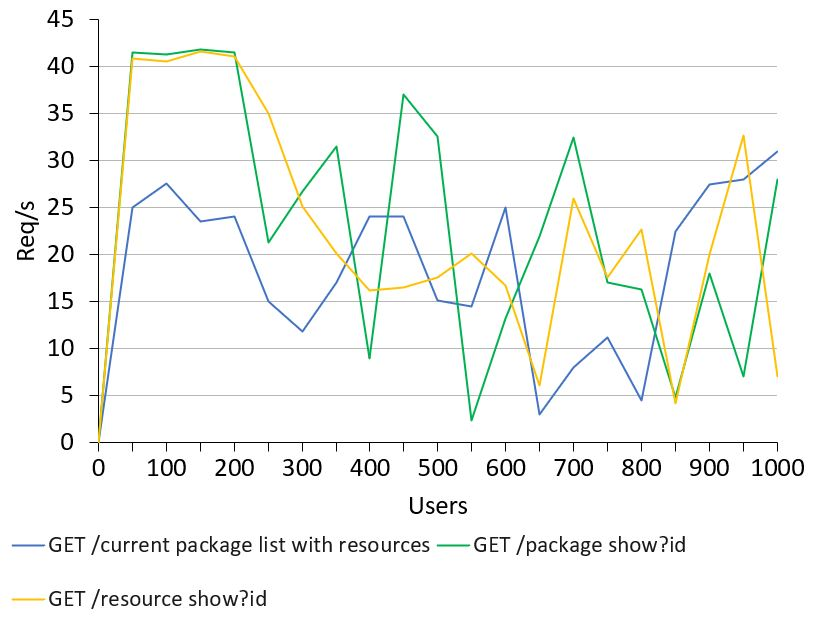
\includegraphics[width=.69\textwidth]{img/performance_evaluation/datasets_individuais.JPG}
    \caption{\label{tab:throughput_datasets}Throughput for dataset and resource requests}
  \end{figure}
  
  
  \begin{figure}[H]
    \centering
    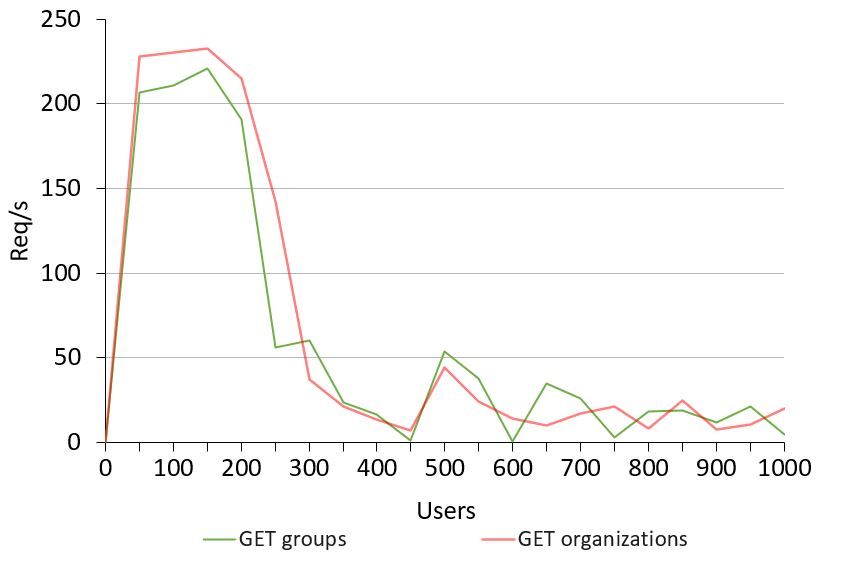
\includegraphics[width=.7\textwidth]{img/performance_evaluation/groups_organizations_individuais.JPG}
    \caption{\label{tab:throughput_groups_org}Throughput for group and organization requests}
  \end{figure}
  
  From the graphs in Figure \ref{tab:throughput_datasets} and \ref{tab:throughput_groups_org}, we can draw some conclusions:
  
  \begin{itemize}
      \item The requests per second increase up to 50 concurrent users, and remain without significant changes up to 200 users, which for now shows to be an interesting data to identify the limit of clients per server from which we will have finished the diminishing returns, and which would be the ideal number of clients to establish as a limit of clients per server. Furthermore, we can notice that the throughput of the requests to the set of groups and/or organisations is much higher, which lies in the fact that this data is much lighter;
      \item After the 200 user mark, there is a significant decrease in the system's ability to handle that many users, with the system's lower ability to manage the number of users suggesting a greater range in requests made per second, getting several inconsistent peaks. This happens most relevantly for requests to read datasets and resources, since the proportion of requests before and after the 200 users is not as noticeable as for organisations or groups;
      \item It would make sense for the throughput to be higher for reading a given resource compared to a given dataset, since its average response size is smaller than the latter. However, \textit{\gls{ckan}} forces the resource request to an extra computation, i.e., it accesses the dataset it belongs to and checks if it is in the dataset's resource list, if the resource is no longer present, then it is non-existent.
  \end{itemize}
  
  \begin{figure}[H]
    \centering
    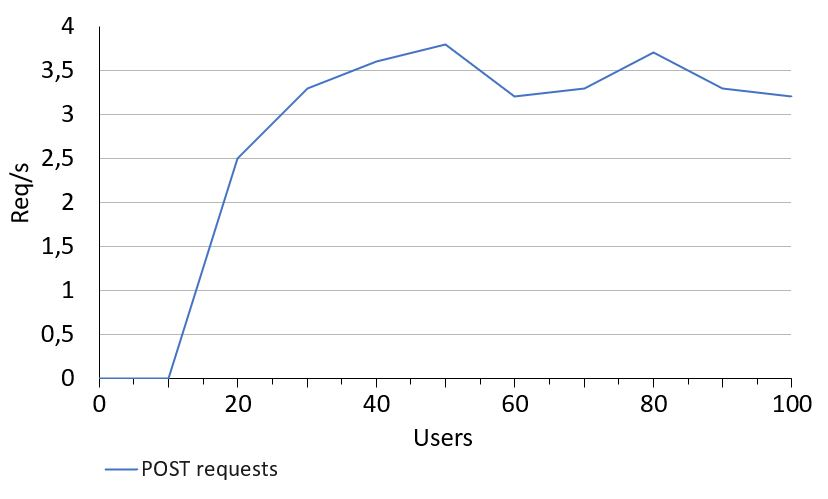
\includegraphics[width=.8\textwidth]{img/performance_evaluation/post_individual.JPG}
    \caption{\label{tab:throughput_write}Throughput for write requests}
  \end{figure}
  
  
  The graph in Figure \ref{tab:throughput_write} shows the huge demand for write requests, being the most relevant bottleneck in this set of requests. Note that the system does not allow to inserting more than one file (resource) at a time, which makes this process even more complex.
  
  
  \subsection{Response time}

  The second metric we sought to analyse was the time it takes the client to receive a response to a given request, distinguishing between each of the types and understanding what factors can influence this response time. As such, we present information in Table \ref{tab:time_individually}.
  
  We chose to analyse only the average time, since, for now, the average time allows us to draw the necessary conclusions for the elaboration of the tests in the following sections.
  
  \newpage
  
    \begin{table}[h]
    \centering
    \begin{tabular}{|>{\centering\arraybackslash}p{6.5cm}|>{\centering\arraybackslash}p{2.5cm}|>{\centering\arraybackslash}p{2cm}|>{\centering\arraybackslash}p{2.5cm}|>{\centering\arraybackslash}p{1cm}|} 
      \hline
      \textbf{Request} & \textbf{\# Requests} & \textbf{Average (ms)} & \textbf{Average size (bytes)} & \textbf{RPS} \\ 
      \hline
      GET /current\_package\_list\_with\_resources & 5178 & 12704 & 216203 & 19.5  \\ 
      \hline
      GET /package\_show?id & 7309 & 9891 & 10603 & 26.8   \\ 
      \hline
      GET /resource\_show?id & 7056 & 10459 & 772 & 25.0    \\
      \hline
      GET /organization\_list & 24350 & 3324 & 129 & 92.5   \\
      \hline
      GET /group\_list & 22222 & 3190 & 116 & 80.6   \\
      \hline
      POST requests & 179 & 9496  & 2178 & 3.5   \\ 
      \hline
    \end{tabular}
    \caption{\label{tab:time_individually}Individual Response Time }
  \end{table}
  
  Analysing Table \ref{tab:time_individually} we can draw three conclusions: 

  \begin{itemize}
    \item The average response time of the server to a given request depends mainly on the size of the response, that is, the smaller the size of the content we want to read, the faster the response will be (even suggesting that we are facing a logarithmic growth) and, consequently, the higher the throughput will also be;
    \item Although for the case of POST requests we consider a smaller sample, it manages to present an average response time almost equal to the reading of datasets with random id's in a sample with 10 times more users. This reinforces the impact that this type of request will have in a real scenario;
    \item The number of requests to the list of organisations is slightly higher than for groups, despite having a larger average size as a response, and we believe this is due to extra calculation that the latter performs, however, we cannot see where this actually happens.
  \end{itemize}
  
  
  \subsection{Summary}
  
  Finally, after these first tests, we can make an overall analysis and make some decisions for those that will follow:
  
  \begin{itemize}
      \item All clients are launched with the same process (running on a single core) by \textit{Locust}, which can end up being limiting when it comes to exploiting the maximum capacity of the available resources, and therefore also when it comes to getting a realistic sense of how the system works. Furthermore, all clients share the network bandwidth, which also limits the throughputs that we collect in these first attempts. However, even though we cannot do anything about the bandwidth sharing, when it comes to using only one core, we will try to exploit the load distribution feature \textit{Locust} has;
      \item Requests that require a random ID of a resource or dataset are time expensive compared to those that use a specific ID, and obviously in a real world scenario this would not happen, but for testing purposes the extra computation generating a random ID is needed. The system may have numerous resources and datasets and each with completely different sizes, so going the other way, such as a default ID, would be misleading; 
      \item In a realistic world scenario a user will not be making requests all the time with no break in between, so we will explore the wait between requests;
      \item \textit{\gls{ckan}} uses pagination when making datasets available to the user through the UI, as such it only loads x number of datasets (by default 20) which enables the insertion of a larger volume of data. We were able to reproduce the same pagination behavior in a similar way, and although we considered increasing the number of datasets in the system, we chose not to do so because as we can see from these early graphs, there is already a considerable amplitude difference between requests early on. However, due to paging, we believe that we could increase the number of data, with slight consequences up to 200 users and bigger problems thereafter. 
  \end{itemize}